%% abtex2-modelo-trabalho-academico.tex, v-1.9.7 laurocesar
%% Copyright 2012-2018 by abnTeX2 group at http://www.abntex.net.br/ 
%%
%% This work may be distributed and/or modified under the
%% conditions of the LaTeX Project Public License, either version 1.3
%% of this license or (at your option) any later version.
%% The latest version of this license is in
%%   http://www.latex-project.org/lppl.txt
%% and version 1.3 or later is part of all distributions of LaTeX
%% version 2005/12/01 or later.
%%
%% This work has the LPPL maintenance status `maintained'.
%% 
%% The Current Maintainer of this work is the abnTeX2 team, led
%% by Lauro César Araujo. Further information are available on 
%% http://www.abntex.net.br/
%%
%% This work consists of the files abntex2-modelo-trabalho-academico.tex,
%% abntex2-modelo-include-comandos and abntex2-modelo-references.bib
%%

% ------------------------------------------------------------------------
% ------------------------------------------------------------------------
% abnTeX2: Modelo de Trabalho Academico (tese de doutorado, dissertacao de
% mestrado e trabalhos monograficos em geral) em conformidade com 
% ABNT NBR 14724:2011: Informacao e documentacao - Trabalhos academicos -
% Apresentacao
% ------------------------------------------------------------------------
% ------------------------------------------------------------------------

\documentclass[
	% -- opções da classe memoir --
	12pt,				% tamanho da fonte
%	openright,			% capítulos começam em pág ímpar (insere página vazia caso preciso)
%	twoside,			% para impressão em recto e verso. Oposto a oneside
	oneside,
	a4paper,			% tamanho do papel. 
	% -- opções da classe abntex2 --
	%chapter=TITLE,		% títulos de capítulos convertidos em letras maiúsculas
	%section=TITLE,		% títulos de seções convertidos em letras maiúsculas
	%subsection=TITLE,	% títulos de subseções convertidos em letras maiúsculas
	%subsubsection=TITLE,% títulos de subsubseções convertidos em letras maiúsculas
	% -- opções do pacote babel --
	english,			% idioma adicional para hifenização
	spanish,			% idioma adicional para hifenização
	brazil				% o último idioma é o principal do documento
	]{abntex2}

% ---
% Pacotes básicos 
% ---
\usepackage{lmodern}			% Usa a fonte Latin Modern			
\usepackage[T1]{fontenc}		% Selecao de codigos de fonte.
\usepackage[utf8]{inputenc}		% Codificacao do documento (conversão automática dos acentos)
\usepackage{indentfirst}		% Indenta o primeiro parágrafo de cada seção.
\usepackage{color}				% Controle das cores
\usepackage{graphicx}			% Inclusão de gráficos
\usepackage{caption}
%\usepackage{longfigure}
\usepackage{subcaption}
%\usepackage[caption = false]{subfig}
\graphicspath{{images/}{../images/}}
\usepackage{longtable}
\usepackage{microtype} 			% para melhorias de justificação
\usepackage{lscape} % para colocar conteúdo (e.g. Imagens) em modo paisagem
\usepackage{enumitem} % para usar algarismos romanos em listas ordenadas
\usepackage{geometry}
\usepackage{pdfpages}
% ---
		
% ---
% Pacotes adicionais, usados apenas no âmbito do Modelo Canônico do abnteX2
% ---
\usepackage{lipsum}				% para geração de dummy text
% ---

% ---
% Pacotes de citações
% ---
\usepackage[brazilian,hyperpageref]{backref}	 % Paginas com as citações na bibl
\usepackage[alf]{abntex2cite}	% Citações padrão ABNT


%Pacote para usar multiplos arquivos
\usepackage{subfiles} % Importa outros arquivos no arquivo tex principal

% --- 
% CONFIGURAÇÕES DE PACOTES
% --- 
% ---
% Configurações do pacote backref
% Usado sem a opção hyperpageref de backref
\renewcommand{\backrefpagesname}{Citado na(s) página(s):~}
% Texto padrão antes do número das páginas
\renewcommand{\backref}{}
% Define os textos da citação
\renewcommand*{\backrefalt}[4]{
	\ifcase #1 %
		Nenhuma citação no texto.%
	\or
		Citado na página #2.%
	\else
		Citado #1 vezes nas páginas #2.%
	\fi}%
% ---
\hyphenation{Pseu-do-myr-me-ci-nae}
% ---
% Informações de dados para CAPA e FOLHA DE ROSTO
% ---
\titulo{ O “FADO DA HERANÇA”: A PÓS-MEMÓRIA DA DITADURA SALAZARISTA EM TRÊS ROMANCES PORTUGUESES PÓS-2000}
\autor{ÁGATA CRISTINA DA SILVA OLIVEIRA}
\local{Rio de Janeiro}
\data{Outubro de 2021}
\orientador{Drª. Gumercinda Nascimento Gonda}
%\coorientador{Equipe \abnTeX}
\instituicao{%
  Ministério da Educação
  \par
  Universidade Federal do Rio de Janeiro 
  \par
  Instituto de Bioquímica Médica Leopoldo de Meis
  }
\tipotrabalho{Tese (Doutorado)}
% O preambulo deve conter o tipo do trabalho, o objetivo, 
% o nome da instituição e a área de concentração 
\preambulo{Tese de doutoramento apresentada ao Programa de PósGraduação em Letras Vernáculas da Faculdade de Letras da Universidade Federal do Rio de Janeiro como requisito para obtenção do título de doutor em Letras Vernáculas.(Literatura Portuguesa Contemporânea).}
% ---


% ---
% Configurações de aparência do PDF final

% alterando o aspecto da cor azul
\definecolor{blue}{RGB}{41,5,195}

% informações do PDF
\makeatletter
\hypersetup{
     	%pagebackref=true,
		pdftitle={\@title}, 
		pdfauthor={\@author},
    	pdfsubject={\imprimirpreambulo},
	    pdfcreator={LaTeX with abnTeX2},
		pdfkeywords={abnt}{latex}{abntex}{abntex2}{trabalho acadêmico}, 
		colorlinks=true,       		% false: boxed links; true: colored links
    	linkcolor=blue,          	% color of internal links
    	citecolor=blue,        		% color of links to bibliography
    	filecolor=magenta,      		% color of file links
		urlcolor=blue,
		bookmarksdepth=4
}
\makeatother
% --- 

% ---
% Posiciona figuras e tabelas no topo da página quando adicionadas sozinhas
% em um página em branco. Ver https://github.com/abntex/abntex2/issues/170
\makeatletter
\setlength{\@fptop}{5pt} % Set distance from top of page to first float
\makeatother
% ---

% ---
% Possibilita criação de Quadros e Lista de quadros.
% Ver https://github.com/abntex/abntex2/issues/176
%
\newcommand{\quadroname}{Quadro}
\newcommand{\listofquadrosname}{Lista de quadros}

\newfloat[chapter]{quadro}{loq}{\quadroname}
\newlistof{listofquadros}{loq}{\listofquadrosname}
\newlistentry{quadro}{loq}{0}

% configurações para atender às regras da ABNT
\setfloatadjustment{quadro}{\centering}
\counterwithout{quadro}{chapter}
\renewcommand{\cftquadroname}{\quadroname\space} 
\renewcommand*{\cftquadroaftersnum}{\hfill--\hfill}
\renewcommand{\listadesiglasname}{Lista de Abreviaturas e Siglas}

\setfloatlocations{quadro}{hbtp} % Ver https://github.com/abntex/abntex2/issues/176
% ---

% --- 
% Espaçamentos entre linhas e parágrafos 
% --- 

% O tamanho do parágrafo é dado por:
\setlength{\parindent}{1.3cm}

% Controle do espaçamento entre um parágrafo e outro:
\setlength{\parskip}{0.2cm}  % tente também \onelineskip

% ---
% compila o indice
% ---
\makeindex
% ---

% ----
% Início do documento
% ----
\begin{document}

% Seleciona o idioma do documento (conforme pacotes do babel)
%\selectlanguage{english}
\selectlanguage{brazil}

% Retira espaço extra obsoleto entre as frases.
\frenchspacing 

% ----------------------------------------------------------
% ELEMENTOS PRÉ-TEXTUAIS
% ----------------------------------------------------------
% \pretextual

% ---
% Capa
% ---
\imprimircapa
% ---

% ---
% Folha de rosto
% (o * indica que haverá a ficha bibliográfica)
% ---
\imprimirfolhaderosto*
% ---

% ---
% Inserir a ficha bibliografica
% ---

% Isto é um exemplo de Ficha Catalográfica, ou ``Dados internacionais de
% catalogação-na-publicação''. Você pode utilizar este modelo como referência. 
% Porém, provavelmente a biblioteca da sua universidade lhe fornecerá um PDF
% com a ficha catalográfica definitiva após a defesa do trabalho. Quando estiver
% com o documento, salve-o como PDF no diretório do seu projeto e substitua todo
% o conteúdo de implementação deste arquivo pelo comando abaixo:
%
% \begin{fichacatalografica}
%     \includepdf{fig_ficha_catalografica.pdf}
% \end{fichacatalografica}

\begin{fichacatalografica}
	\sffamily
	\vspace*{\fill}					% Posição vertical
	\begin{center}					% Minipage Centralizado
	\fbox{\begin{minipage}[c][8cm]{13.5cm}		% Largura
	\small
	\imprimirautor
	%Sobrenome, Nome do autor
	
	\hspace{0.5cm} \imprimirtitulo  / \imprimirautor. --
	\imprimirlocal, \imprimirdata-
	
	\hspace{0.5cm} \thelastpage p. : il. (algumas color.) ; 30 cm.\\
	
	\hspace{0.5cm} \imprimirorientadorRotulo~\imprimirorientador\\
	
	\hspace{0.5cm}
	\parbox[t]{\textwidth}{\imprimirtipotrabalho~--~\imprimirinstituicao,
	\imprimirdata.}\\
	
	\hspace{0.5cm}
		1. Palavra-chave1.
		2. Palavra-chave2.
		2. Palavra-chave3.
		I. Orientador.
		II. Universidade xxx.
		III. Faculdade de xxx.
		IV. Título 			
	\end{minipage}}
	\end{center}
\end{fichacatalografica}
% ---

% ---
% Inserir errata
% ---
%\begin{errata}
%Elemento opcional da \citeonline[4.2.1.2]{NBR14724:2011}. Exemplo:

%\vspace{\onelineskip}

%FERRIGNO, C. R. A. \textbf{Tratamento de neoplasias ósseas apendiculares com
%reimplantação de enxerto ósseo autólogo autoclavado associado ao plasma
%rico em plaquetas}: estudo crítico na cirurgia de preservação de membro em
%cães. 2011. 128 f. Tese (Livre-Docência) - Faculdade de Medicina Veterinária e
%Zootecnia, Universidade de São Paulo, São Paulo, 2011.

%\begin{table}[htb]
%\center
%\footnotesize
%\begin{tabular}{|p{1.4cm}|p{1cm}|p{3cm}|p{3cm}|}
% \hline
% \textbf{Folha} & \textbf{Linha}  & \textbf{Onde se lê}  & \textbf{Leia-se}  \\
%  \hline
%    1 & 10 & auto-conclavo & autoconclavo\\
%   \hline
%\end{tabular}
%\end{table}

%\end{errata}
% ---

% ---
% Inserir folha de aprovação
% ---

% Isto é um exemplo de Folha de aprovação, elemento obrigatório da NBR
% 14724/2011 (seção 4.2.1.3). Você pode utilizar este modelo até a aprovação
% do trabalho. Após isso, substitua todo o conteúdo deste arquivo por uma
% imagem da página assinada pela banca com o comando abaixo:
%
% \begin{folhadeaprovacao}
% \includepdf{folhadeaprovacao_final.pdf}
% \end{folhadeaprovacao}
%
\begin{folhadeaprovacao}

\begin{center}
      \ABNTEXchapterfont\imprimirtitulo
      \vspace{\fill}
      \ABNTEXchapterfont\large\imprimirautor
      \vspace{\fill}
	\begin{flushleft}
		\ABNTEXchapterfont\large\imprimirpreambulo\vfill
		 
		Aprovado em: 26/03/2019
	\end{flushleft}
	BANCA EXAMINADORA
	\vspace{\fill}
	\hrule\textbf{\imprimirorientador} \\ Prof. Adjunto do Instituto de Bioquímica Médica Leopoldo de Meis da Universidade Federal do Rio de Janeiro – UFRJ
	\vspace{\fill}
	\hrule\textbf{Drª. Carla Ribeiro Polycarpo} \\ Profª. Associada do Instituto de Bioquímica Médica Leopoldo de Meis da Universidade Federal do Rio de Janeiro – UFRJ
	\vspace{\fill}
	\hrule\textbf{Drª Ana Carolina Martins Junqueira} \\ Profª. Adjunta do Instituto de Bioquímica Médica Leopoldo de Meis da Universidade Federal do Rio de Janeiro – UFRJ
	\vspace{\fill}
	\hrule\textbf{Dr. Marcus Fernandes de Oliveira} \\ Prof. Adjunto do Instituto de Bioquímica Médica Leopoldo de Meis da Universidade Federal do Rio de Janeiro – UFRJ
	\vspace{\fill}
	\hrule\textbf{Suplente externo: Dr. Marcelo Weksler} \\ Prof. Titular do Programa de Pós-Graduação em Zoologia do Museu Nacional da Universidade Federal do Rio de Janeiro - UFRJ
	\vspace{\fill}
	\hrule\textbf{Revisor: Dr.  Fernando Lucas Palhano Soares} \\ Prof. Adjunto do Instituto de Bioquímica Médica Leopoldo de Meis da Universidade Federal do Rio de Janeiro – UFRJ \\
\end{center}
  
\end{folhadeaprovacao}
% ---

% ---
% Dedicatória
% ---
%\begin{dedicatoria}
%   \vspace*{\fill}
%   \centering
%   \noindent
%   \textit{ Este trabalho é dedicado às crianças adultas que,\\
%   quando pequenas, sonharam em se tornar cientistas.} \vspace*{\fill}
%\end{dedicatoria}
% ---

% ---
% Agradecimentos
% ---
\begin{agradecimentos}
Agradeço a minha mãe por ter me inserido no mundo dos livros. Por ter me apresentado aos sebos, aos clássicos da literatura brasileira e a Paulo Freire. Agradeço por cada dia que ficava me esperando chegar no último ônibus, sei bem que com o coração na mão, e me obrigava a jantar, sempre desconfiada que com a minha rotina de trabalho durante o dia em Japeri e UFF à noite em Niterói eu não estivesse comendo direito. E sentava à mesa comigo e ouvia pacientemente, à uma da manhã, eu contar sobre o meu dia. Agradeço por depositar tanta confiança em mim que faz com que eu me sinta confiante.

Ao meu amado companheiro Gabriel, a pessoa cuja vida mais se entrelaça com a escrita desta tese. Deixou para trás seu estado e sua universidade de origem para me acompanhar. Não deixou que minha crise de ansiedade fizesse com que eu desistisse da entrevista para o doutorado. Segurou minhas mãos em todas as crises de ansiedade seguintes que quase fizeram com que eu desistisse de tudo. Tomo emprestadas as palavras de Saramago em Manual de Pintura e Caligrafia para dizer que “não vieste nem cedo nem tarde. Vieste na hora certa, no minuto exacto, no preciso e precioso patamar do tempo em que eu podia esperar-te”.

À minha querida orientadora e amiga Cinda tenho tantas coisas a agradecer que nem sei por onde começar. Talvez a coisa mais importante seja o modelo de mulher forte, empática e diligente que deixa para mim. Espero poder fazer aos outros tudo o que você fez por mim.

Aos meus queridos companheiros de orientação Aline, Luana, Luciana e Paulo por todas as conversas, trocas de ideias, risadas, lágrimas, tantas coisas que compartilhamos que fazem com que eu não consiga imaginar a vida sem vocês.

Aos queridos membros da banca agradeço por seus olhares atentos e por serem tão generosos a ponto de tomarem tempo para ler e refletir sobre esta tese. 

À todos os funcionários da UFRJ que contribuem para que tudo funcione dentro da universidade e proporcionam um ambiente limpo e agradável.

Aos presidentes Lula e Dilma pelas políticas que permitiram com que eu fosse fazer parte da minha graduação na Universidade de Coimbra e ampliasse meus conhecimentos de mundo. Talvez sem isso eu nem sequer tivesse conhecido meus objetos de estudo. Talvez tudo fosse completamente diferente na minha vida.

À FAPERJ agradeço pelo financiamento desta pesquisa através da Bolsa Nota 10.

\end{agradecimentos}
% ---

% ---
% Epígrafe
% ---
\begin{epigrafe}
    \vspace*{\fill}
	\begin{flushright}
		\textit{
		``Non omnis moriar'' \\
		(Horácio. Odes, III, 30, 6)
	}
	\end{flushright}
\end{epigrafe}
% ---

% ---
% RESUMOS
% ---

% resumo em português
\setlength{\absparsep}{18pt} % ajusta o espaçamento dos parágrafos do resumo
\begin{resumo}
O “fado da herança”: a pós-memória da ditadura salazarista em três romances portugueses pós-2000

Resumo da tese de doutoramento apresentada ao Programa de Pós-Graduação em Letras Vernáculas da Faculdade de Letras da Universidade Federal do Rio de Janeiro como requisito para obtenção do título de doutor em Letras Vernáculas. (Literatura Portuguesa). 

Oliveira, Ágata Cristina da Silva. O “fado da herança”: a pós-memória da ditadura salazarista em três romances portugueses pós-2000. Rio de Janeiro, 2021. (doutoramento em Literatura Portuguesa). Faculdade de Letras, Universidade Federal do Rio de Janeiro. Rio de Janeiro, 2021.


A presente tese intitulada “O “fado da herança”: a pós-memória da ditadura salazarista em três romances portugueses pós-2000” propõe-se a analisar os romances Deixem falar as pedras (2011), de David Machado, Anatomia dos Mártires (2011), de João Tordo e O teu rosto será o último (2012), de João Ricardo Pedro. O objetivo desta tese é, através da análise comparativa de três romances de três autores portugueses da geração após 2000, apontar para as formas como se escrevem as heranças histórica e literária oriundas das gerações que vivenciaram o período do Estado Novo em Portugal. Para tal, apontar-se-á, sobretudo, para o papel dos narradores e a forma empregada em cada texto a fim de refletir uma escrita da pós-memória. 

Entre os referenciais teóricos estão os textos The generation of postmemory: writing and visual culture after the holocaust, de Marianne Hirsch, Espaços da recordação, de Aleida Assmann, Mutações da literatura no século XXI, de Leyla Perrone-Moisés, Heterodoxia II, de Eduardo Lourenço, Espectros de Marx, de Jacques Derrida, Problemas da poética de Dostoiévski, de Mikhail Bakhtin, O labirinto da saudade, de Eduardo Lourenço, O anjo da história, de Walter Benjamin, A alma e as formas, Georg Lukács, entre outros. 



 \textbf{Palavras-chave}: Literatura portuguesa. Literatura e Memória. David Machado. João Tordo. João Ricardo Pedro.
\end{resumo}

% resumo em inglês
\begin{resumo}[Abstract]
 \begin{otherlanguage*}{english}
   
   Summary of doctoral thesis presented to the Graduate Program in vernacular letters of the Faculdade de Letras da Universidade Federal do Rio de Janeiro as a requirement for obtaining the title of Doctor of Letters vernacular. (Portuguese Literature). 
   Oliveira, Ágata Cristina da Silva.  Rio de Janeiro, 2021. (Doctorate in Portuguese Literature). Faculty of Letters, Federal University of Rio de Janeiro. Rio de Janeiro, 2021.
   
   \vspace{\onelineskip}
 
   \noindent 
   \textbf{Keywords}: Pseudomyrmecinae, Mitogenomics, Data mining, Bioinformatics, Phylogenomics, Ant evolutionary biology, Next Generation Sequencing, Public data. 
 \end{otherlanguage*}
\end{resumo}

% resumo em francês 
%\begin{resumo}[Résumé]
% \begin{otherlanguage*}{french}
%    Il s'agit d'un résumé en français.
% 
%   \textbf{Mots-clés}: latex. abntex. publication de textes.
% \end{otherlanguage*}
%\end{resumo}

% resumo em espanhol
%\begin{resumo}[Resumen]
% \begin{otherlanguage*}{spanish}
%   Este es el resumen en español.
  
%   \textbf{Palabras clave}: latex. abntex. publicación de textos.
% \end{otherlanguage*}
%\end{resumo}
% ---

% ---
% inserir lista de ilustrações
% ---
\pdfbookmark[0]{\listfigurename}{lof}
\listoffigures*
\cleardoublepage
% ---

% ---
% inserir lista de quadros
% ---
%\pdfbookmark[0]{\listofquadrosname}{loq}
%\listofquadros*
%\cleardoublepage
% ---

% ---
% inserir lista de tabelas
% ---
\pdfbookmark[0]{\listtablename}{lot}
\listoftables*
\cleardoublepage
% ---

% ---
% inserir lista de abreviaturas e siglas
% ---
%\begin{siglas}
%  \item[\textbf{3’OH:}] Hidroxila presente no carbono 3’ de um nucleotídeo
%  \item[\textbf{A:}] Amina (base púrica)
%  \item[\textbf{ATP6:}] ATP sintase F0 subunidade 6
%  \item[\textbf{ATP8:}] ATP sintase F0 subunidade 8
%  \item[\textbf{BLAST:}] Basic Local Alignment Search Tool
%  \item[\textbf{BLASTp:}] Protein-protein BLAST
%  \item[\textbf{BRIG:}] Blast Ring Image Generator
%  \item[\textbf{BS:}] Suporte de Bootstrap
%\end{siglas}

% ---

% ---
% inserir lista de símbolos
% ---
%\begin{simbolos}
%  \item[$ \Gamma $] Letra grega Gama
%  \item[$ \Lambda $] Lambda
%  \item[$ \zeta $] Letra grega minúscula zeta
%  \item[$ \in $] Pertence
%\end{simbolos}
% ---

% ---
% inserir o sumario
% ---
\pdfbookmark[0]{\contentsname}{toc}
\tableofcontents*
\cleardoublepage
% ---



% ----------------------------------------------------------
% ELEMENTOS TEXTUAIS
% ----------------------------------------------------------
\textual

% ----------------------------------------------------------
% Introdução (exemplo de capítulo sem numeração, mas presente no Sumário)
% ----------------------------------------------------------
\chapter*[Introduction. QUANDO ME ENCONTRO NO CALOR DA LUTA]{ “QUANDO ME ENCONTRO NO CALOR DA LUTA”}
\addcontentsline{toc}{chapter}{ “QUANDO ME ENCONTRO NO CALOR DA LUTA”}

\subfile{TESE_CAPITULOS/INTRODUCAO}

% ----------------------------------------------------------

\chapter[“TIVE, PORÉM, QUE LEMBRAR O MEU PASSADO”]{“TIVE, PORÉM, QUE LEMBRAR O MEU PASSADO”: NO ENTORNO DO 25 DE ABRIL}

\subfile{TESE_CAPITULOS/CAPITULO_1}

\chapter{Metodologia}

%\subfile{TESE_CAPITULOS/03_METODOS}

\chapter{Resultados}

%\subfile{TESE_CAPITULOS/04_RESULTADOS}

\chapter{Discussão}

%\subfile{TESE_CAPITULOS/05_DISCUSSAO}

\chapter{Perspectivas}

%\subfile{TESE_CAPITULOS/06_PERSPECTIVAS}

\chapter{Conclusão}

%\subfile{TESE_CAPITULOS/07_CONCLUSAO}

% ---
% ----------------------------------------------------------
% ELEMENTOS PÓS-TEXTUAIS
% ----------------------------------------------------------
\postextual
% ----------------------------------------------------------

% ----------------------------------------------------------
% Referências bibliográficas
% ----------------------------------------------------------
%\bibliography{library}\label{references}

% ----------------------------------------------------------
% Glossário
% ----------------------------------------------------------
%
% Consulte o manual da classe abntex2 para orientações sobre o glossário.
%
%\glossary

% ----------------------------------------------------------
% Apêndices
% ----------------------------------------------------------

% ---
% Inicia os apêndices
% ---
\begin{apendicesenv}

% Imprime uma página indicando o início dos apêndices
\partapendices

% ----------------------------------------------------------
\chapter{Figuras e tabelas adicionais}
% ----------------------------------------------------------

%\subfile{TESE_CAPITULOS/08_APENDICESA}

% ----------------------------------------------------------
%\chapter{Artigo publicado}
% ----------------------------------------------------------

\chapter{Artigo Publicado}

%\includepdf[pages={2-}]{TESE_CAPITULOS/08_APENDICESB.pdf}

\end{apendicesenv}
% ---


% ----------------------------------------------------------
% Anexos
% ----------------------------------------------------------

% ---
% Inicia os anexos
% ---
%\begin{anexosenv}

% Imprime uma página indicando o início dos anexos
%\partanexos

% ---
%\chapter{Morbi ultrices rutrum lorem.}
% ---
%\lipsum[30]

% ---
%\chapter{Cras non urna sed feugiat cum sociis natoque penatibus et magnis dis
%parturient montes nascetur ridiculus mus}
% ---

%\lipsum[31]

% ---
%\chapter{Fusce facilisis lacinia dui}
% ---

%\lipsum[32]

%\end{anexosenv}

%---------------------------------------------------------------------
% INDICE REMISSIVO
%---------------------------------------------------------------------
\phantompart
\printindex
%---------------------------------------------------------------------

\end{document}
